\documentclass[1p]{elsarticle_modified}
%\bibliographystyle{elsarticle-num}

%\usepackage[colorlinks]{hyperref}
%\usepackage{abbrmath_seonhwa} %\Abb, \Ascr, \Acal ,\Abf, \Afrak
\usepackage{amsfonts}
\usepackage{amssymb}
\usepackage{amsmath}
\usepackage{amsthm}
\usepackage{scalefnt}
\usepackage{amsbsy}
\usepackage{kotex}
\usepackage{caption}
\usepackage{subfig}
\usepackage{color}
\usepackage{graphicx}
\usepackage{xcolor} %% white, black, red, green, blue, cyan, magenta, yellow
\usepackage{float}
\usepackage{setspace}
\usepackage{hyperref}

\usepackage{tikz}
\usetikzlibrary{arrows}

\usepackage{multirow}
\usepackage{array} % fixed length table
\usepackage{hhline}

%%%%%%%%%%%%%%%%%%%%%
\makeatletter
\renewcommand*\env@matrix[1][\arraystretch]{%
	\edef\arraystretch{#1}%
	\hskip -\arraycolsep
	\let\@ifnextchar\new@ifnextchar
	\array{*\c@MaxMatrixCols c}}
\makeatother %https://tex.stackexchange.com/questions/14071/how-can-i-increase-the-line-spacing-in-a-matrix
%%%%%%%%%%%%%%%

\usepackage[normalem]{ulem}

\newcommand{\msout}[1]{\ifmmode\text{\sout{\ensuremath{#1}}}\else\sout{#1}\fi}
%SOURCE: \msout is \stkout macro in https://tex.stackexchange.com/questions/20609/strikeout-in-math-mode

\newcommand{\cancel}[1]{
	\ifmmode
	{\color{red}\msout{#1}}
	\else
	{\color{red}\sout{#1}}
	\fi
}

\newcommand{\add}[1]{
	{\color{blue}\uwave{#1}}
}

\newcommand{\replace}[2]{
	\ifmmode
	{\color{red}\msout{#1}}{\color{blue}\uwave{#2}}
	\else
	{\color{red}\sout{#1}}{\color{blue}\uwave{#2}}
	\fi
}

\newcommand{\Sol}{\mathcal{S}} %segment
\newcommand{\D}{D} %diagram
\newcommand{\A}{\mathcal{A}} %arc


%%%%%%%%%%%%%%%%%%%%%%%%%%%%%5 test

\def\sl{\operatorname{\textup{SL}}(2,\Cbb)}
\def\psl{\operatorname{\textup{PSL}}(2,\Cbb)}
\def\quan{\mkern 1mu \triangleright \mkern 1mu}

\theoremstyle{definition}
\newtheorem{thm}{Theorem}[section]
\newtheorem{prop}[thm]{Proposition}
\newtheorem{lem}[thm]{Lemma}
\newtheorem{ques}[thm]{Question}
\newtheorem{cor}[thm]{Corollary}
\newtheorem{defn}[thm]{Definition}
\newtheorem{exam}[thm]{Example}
\newtheorem{rmk}[thm]{Remark}
\newtheorem{alg}[thm]{Algorithm}

\newcommand{\I}{\sqrt{-1}}
\begin{document}

%\begin{frontmatter}
%
%\title{Boundary parabolic representations of knots up to 8 crossings}
%
%%% Group authors per affiliation:
%\author{Yunhi Cho} 
%\address{Department of Mathematics, University of Seoul, Seoul, Korea}
%\ead{yhcho@uos.ac.kr}
%
%
%\author{Seonhwa Kim} %\fnref{s_kim}}
%\address{Center for Geometry and Physics, Institute for Basic Science, Pohang, 37673, Korea}
%\ead{ryeona17@ibs.re.kr}
%
%\author{Hyuk Kim}
%\address{Department of Mathematical Sciences, Seoul National University, Seoul 08826, Korea}
%\ead{hyukkim@snu.ac.kr}
%
%\author{Seokbeom Yoon}
%\address{Department of Mathematical Sciences, Seoul National University, Seoul, 08826,  Korea}
%\ead{sbyoon15@snu.ac.kr}
%
%\begin{abstract}
%We find all boundary parabolic representation of knots up to 8 crossings.
%
%\end{abstract}
%\begin{keyword}
%    \MSC[2010] 57M25 
%\end{keyword}
%
%\end{frontmatter}

%\linenumbers
%\tableofcontents
%
\newcommand\colored[1]{\textcolor{white}{\rule[-0.35ex]{0.8em}{1.4ex}}\kern-0.8em\color{red} #1}%
%\newcommand\colored[1]{\textcolor{white}{ #1}\kern-2.17ex	\textcolor{white}{ #1}\kern-1.81ex	\textcolor{white}{ #1}\kern-2.15ex\color{red}#1	}

{\Large $\underline{12n_{0413}~(K12n_{0413})}$}

\setlength{\tabcolsep}{10pt}
\renewcommand{\arraystretch}{1.6}
\vspace{1cm}\begin{tabular}{m{100pt}>{\centering\arraybackslash}m{274pt}}
\multirow{5}{120pt}{
	\centering
	\includegraphics[width=112pt]{../../../GIT/diagram.site/Diagrams/png/2502_12n_0413.png}\\
\ \ \ A knot diagram\footnotemark}&
\allowdisplaybreaks
\textbf{Linearized knot diagam} \\
\cline{2-2}
 &
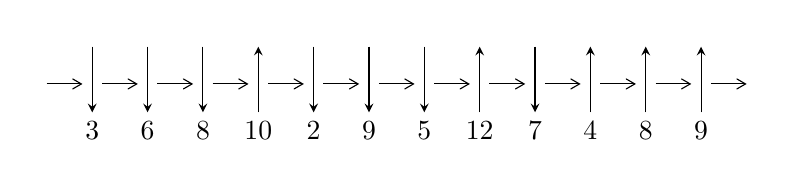
\begin{tikzpicture}[x=20pt, y=17pt]
	% nodes
	\node (C0) at (0, 0) {};
	\node (C1) at (1, 0) {};
	\node (C1U) at (1, +1) {};
	\node (C1D) at (1, -1) {3};

	\node (C2) at (2, 0) {};
	\node (C2U) at (2, +1) {};
	\node (C2D) at (2, -1) {6};

	\node (C3) at (3, 0) {};
	\node (C3U) at (3, +1) {};
	\node (C3D) at (3, -1) {8};

	\node (C4) at (4, 0) {};
	\node (C4U) at (4, +1) {};
	\node (C4D) at (4, -1) {10};

	\node (C5) at (5, 0) {};
	\node (C5U) at (5, +1) {};
	\node (C5D) at (5, -1) {2};

	\node (C6) at (6, 0) {};
	\node (C6U) at (6, +1) {};
	\node (C6D) at (6, -1) {9};

	\node (C7) at (7, 0) {};
	\node (C7U) at (7, +1) {};
	\node (C7D) at (7, -1) {5};

	\node (C8) at (8, 0) {};
	\node (C8U) at (8, +1) {};
	\node (C8D) at (8, -1) {12};

	\node (C9) at (9, 0) {};
	\node (C9U) at (9, +1) {};
	\node (C9D) at (9, -1) {7};

	\node (C10) at (10, 0) {};
	\node (C10U) at (10, +1) {};
	\node (C10D) at (10, -1) {4};

	\node (C11) at (11, 0) {};
	\node (C11U) at (11, +1) {};
	\node (C11D) at (11, -1) {8};

	\node (C12) at (12, 0) {};
	\node (C12U) at (12, +1) {};
	\node (C12D) at (12, -1) {9};
	\node (C13) at (13, 0) {};

	% arrows
	\draw[->,>={angle 60}]
	(C0) edge (C1) (C1) edge (C2) (C2) edge (C3) (C3) edge (C4) (C4) edge (C5) (C5) edge (C6) (C6) edge (C7) (C7) edge (C8) (C8) edge (C9) (C9) edge (C10) (C10) edge (C11) (C11) edge (C12) (C12) edge (C13) ;	\draw[->,>=stealth]
	(C1U) edge (C1D) (C2U) edge (C2D) (C3U) edge (C3D) (C4D) edge (C4U) (C5U) edge (C5D) (C6U) edge (C6D) (C7U) edge (C7D) (C8D) edge (C8U) (C9U) edge (C9D) (C10D) edge (C10U) (C11D) edge (C11U) (C12D) edge (C12U) ;
	\end{tikzpicture} \\
\hhline{~~} \\& 
\textbf{Solving Sequence} \\ \cline{2-2} 
 &
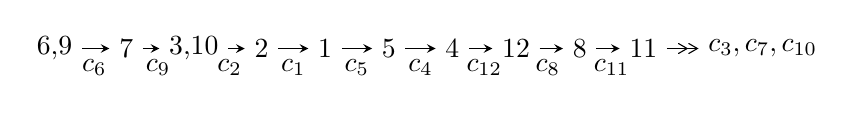
\begin{tikzpicture}[x=23pt, y=7pt]
	% node
	\node (A0) at (-1/8, 0) {6,9};
	\node (A1) at (1, 0) {7};
	\node (A2) at (33/16, 0) {3,10};
	\node (A3) at (25/8, 0) {2};
	\node (A4) at (33/8, 0) {1};
	\node (A5) at (41/8, 0) {5};
	\node (A6) at (49/8, 0) {4};
	\node (A7) at (57/8, 0) {12};
	\node (A8) at (65/8, 0) {8};
	\node (A9) at (73/8, 0) {11};
	\node (C1) at (1/2, -1) {$c_{6}$};
	\node (C2) at (3/2, -1) {$c_{9}$};
	\node (C3) at (21/8, -1) {$c_{2}$};
	\node (C4) at (29/8, -1) {$c_{1}$};
	\node (C5) at (37/8, -1) {$c_{5}$};
	\node (C6) at (45/8, -1) {$c_{4}$};
	\node (C7) at (53/8, -1) {$c_{12}$};
	\node (C8) at (61/8, -1) {$c_{8}$};
	\node (C9) at (69/8, -1) {$c_{11}$};
	\node (A10) at (11, 0) {$c_{3},c_{7},c_{10}$};

	% edge
	\draw[->,>=stealth]	
	(A0) edge (A1) (A1) edge (A2) (A2) edge (A3) (A3) edge (A4) (A4) edge (A5) (A5) edge (A6) (A6) edge (A7) (A7) edge (A8) (A8) edge (A9) ;
	\draw[->>,>={angle 60}]	
	(A9) edge (A10);
\end{tikzpicture} \\ 

\end{tabular} \\

\footnotetext{
The image of knot diagram is generated by the software ``\textbf{Draw programme}" developed by Andrew Bartholomew(\url{http://www.layer8.co.uk/maths/draw/index.htm\#Running-draw}), where we modified some parts for our purpose(\url{https://github.com/CATsTAILs/LinksPainter}).
}\phantom \\ \newline 
\centering \textbf{Ideals for irreducible components\footnotemark of $X_{\text{par}}$} 
 
\begin{align*}
I^u_{1}&=\langle 
-9.68083\times10^{106} u^{48}+1.80477\times10^{107} u^{47}+\cdots+7.70077\times10^{108} b+4.07046\times10^{109},\\
\phantom{I^u_{1}}&\phantom{= \langle  }6.39121\times10^{109} u^{48}-1.62145\times10^{110} u^{47}+\cdots+1.28603\times10^{111} a-1.39682\times10^{112},\\
\phantom{I^u_{1}}&\phantom{= \langle  }u^{49}-2 u^{48}+\cdots-1083 u-167\rangle \\
I^u_{2}&=\langle 
-4356880 u^{16}+8072348 u^{15}+\cdots+14725657 b+19826117,\\
\phantom{I^u_{2}}&\phantom{= \langle  }15345062 u^{16}-28541073 u^{15}+\cdots+14725657 a-99165990,\;u^{17}- u^{16}+\cdots-5 u-1\rangle \\
I^u_{3}&=\langle 
b+1,\;u^3+2 u^2+a-1,\;u^4+3 u^3+2 u^2+1\rangle \\
I^u_{4}&=\langle 
b+1,\;a+2,\;u-1\rangle \\
\\
\end{align*}
\raggedright * 4 irreducible components of $\dim_{\mathbb{C}}=0$, with total 71 representations.\\
\footnotetext{All coefficients of polynomials are rational numbers. But the coefficients are sometimes approximated in decimal forms when there is not enough margin.}
\newpage
\renewcommand{\arraystretch}{1}
\centering \section*{I. $I^u_{1}= \langle -9.68\times10^{106} u^{48}+1.80\times10^{107} u^{47}+\cdots+7.70\times10^{108} b+4.07\times10^{109},\;6.39\times10^{109} u^{48}-1.62\times10^{110} u^{47}+\cdots+1.29\times10^{111} a-1.40\times10^{112},\;u^{49}-2 u^{48}+\cdots-1083 u-167 \rangle$}
\flushleft \textbf{(i) Arc colorings}\\
\begin{tabular}{m{7pt} m{180pt} m{7pt} m{180pt} }
\flushright $a_{6}=$&$\begin{pmatrix}1\\0\end{pmatrix}$ \\
\flushright $a_{9}=$&$\begin{pmatrix}0\\u\end{pmatrix}$ \\
\flushright $a_{7}=$&$\begin{pmatrix}1\\u^2\end{pmatrix}$ \\
\flushright $a_{3}=$&$\begin{pmatrix}-0.0496973 u^{48}+0.126082 u^{47}+\cdots+51.3655 u+10.8615\\0.0125713 u^{48}-0.0234362 u^{47}+\cdots-23.9191 u-5.28578\end{pmatrix}$ \\
\flushright $a_{10}=$&$\begin{pmatrix}- u\\- u^3+u\end{pmatrix}$ \\
\flushright $a_{2}=$&$\begin{pmatrix}-0.0371260 u^{48}+0.102646 u^{47}+\cdots+27.4464 u+5.57574\\0.0125713 u^{48}-0.0234362 u^{47}+\cdots-23.9191 u-5.28578\end{pmatrix}$ \\
\flushright $a_{1}=$&$\begin{pmatrix}-0.0147332 u^{48}+0.0581855 u^{47}+\cdots-5.41058 u+0.310122\\0.0402524 u^{48}-0.122863 u^{47}+\cdots-26.9497 u-3.52830\end{pmatrix}$ \\
\flushright $a_{5}=$&$\begin{pmatrix}-0.0182261 u^{48}+0.0716241 u^{47}+\cdots-6.44692 u-6.24038\\-0.152512 u^{48}+0.408573 u^{47}+\cdots+193.403 u+40.3475\end{pmatrix}$ \\
\flushright $a_{4}=$&$\begin{pmatrix}0.0676174 u^{48}-0.168317 u^{47}+\cdots-101.750 u-24.4584\\-0.182706 u^{48}+0.491490 u^{47}+\cdots+229.123 u+47.1670\end{pmatrix}$ \\
\flushright $a_{12}=$&$\begin{pmatrix}-0.0147332 u^{48}+0.0581855 u^{47}+\cdots-5.41058 u+0.310122\\0.0101824 u^{48}-0.0352370 u^{47}+\cdots+1.69276 u+1.26781\end{pmatrix}$ \\
\flushright $a_{8}=$&$\begin{pmatrix}0.0328901 u^{48}-0.0927795 u^{47}+\cdots-48.5742 u-1.25960\\0.0758750 u^{48}-0.205486 u^{47}+\cdots-90.6780 u-20.9576\end{pmatrix}$ \\
\flushright $a_{11}=$&$\begin{pmatrix}-0.0537472 u^{48}+0.151765 u^{47}+\cdots+60.2707 u+8.53722\\0.0318713 u^{48}-0.0804240 u^{47}+\cdots-41.2502 u-8.00996\end{pmatrix}$\\&\end{tabular}
\flushleft \textbf{(ii) Obstruction class $= -1$}\\~\\
\flushleft \textbf{(iii) Cusp Shapes $= 0.462159 u^{48}-1.17412 u^{47}+\cdots-696.600 u-157.924$}\\~\\
\newpage\renewcommand{\arraystretch}{1}
\flushleft \textbf{(iv) u-Polynomials at the component}\newline \\
\begin{tabular}{m{50pt}|m{274pt}}
Crossings & \hspace{64pt}u-Polynomials at each crossing \\
\hline $$\begin{aligned}c_{1}\end{aligned}$$&$\begin{aligned}
&u^{49}+29 u^{48}+\cdots+3724 u+784
\end{aligned}$\\
\hline $$\begin{aligned}c_{2},c_{5}\end{aligned}$$&$\begin{aligned}
&u^{49}-3 u^{48}+\cdots-70 u+28
\end{aligned}$\\
\hline $$\begin{aligned}c_{3}\end{aligned}$$&$\begin{aligned}
&u^{49}+2 u^{48}+\cdots-3520 u+227
\end{aligned}$\\
\hline $$\begin{aligned}c_{4},c_{10}\end{aligned}$$&$\begin{aligned}
&u^{49}+3 u^{48}+\cdots-60 u+29
\end{aligned}$\\
\hline $$\begin{aligned}c_{6},c_{9}\end{aligned}$$&$\begin{aligned}
&u^{49}+2 u^{48}+\cdots-1083 u+167
\end{aligned}$\\
\hline $$\begin{aligned}c_{7}\end{aligned}$$&$\begin{aligned}
&u^{49}-4 u^{48}+\cdots-400 u+79
\end{aligned}$\\
\hline $$\begin{aligned}c_{8},c_{11},c_{12}\end{aligned}$$&$\begin{aligned}
&u^{49}-5 u^{48}+\cdots+127 u+7
\end{aligned}$\\
\hline
\end{tabular}\\~\\
\newpage\renewcommand{\arraystretch}{1}
\flushleft \textbf{(v) Riley Polynomials at the component}\newline \\
\begin{tabular}{m{50pt}|m{274pt}}
Crossings & \hspace{64pt}Riley Polynomials at each crossing \\
\hline $$\begin{aligned}c_{1}\end{aligned}$$&$\begin{aligned}
&y^{49}-13 y^{48}+\cdots-10750992 y-614656
\end{aligned}$\\
\hline $$\begin{aligned}c_{2},c_{5}\end{aligned}$$&$\begin{aligned}
&y^{49}-29 y^{48}+\cdots+3724 y-784
\end{aligned}$\\
\hline $$\begin{aligned}c_{3}\end{aligned}$$&$\begin{aligned}
&y^{49}-86 y^{48}+\cdots+4342796 y-51529
\end{aligned}$\\
\hline $$\begin{aligned}c_{4},c_{10}\end{aligned}$$&$\begin{aligned}
&y^{49}+61 y^{48}+\cdots-7014 y-841
\end{aligned}$\\
\hline $$\begin{aligned}c_{6},c_{9}\end{aligned}$$&$\begin{aligned}
&y^{49}-48 y^{48}+\cdots+633479 y-27889
\end{aligned}$\\
\hline $$\begin{aligned}c_{7}\end{aligned}$$&$\begin{aligned}
&y^{49}-6 y^{48}+\cdots+26648 y-6241
\end{aligned}$\\
\hline $$\begin{aligned}c_{8},c_{11},c_{12}\end{aligned}$$&$\begin{aligned}
&y^{49}-3 y^{48}+\cdots+7771 y-49
\end{aligned}$\\
\hline
\end{tabular}\\~\\
\newpage\flushleft \textbf{(vi) Complex Volumes and Cusp Shapes}
$$\begin{array}{c|c|c}  
\text{Solutions to }I^u_{1}& \I (\text{vol} + \sqrt{-1}CS) & \text{Cusp shape}\\
 \hline 
\begin{aligned}
u &= -0.850931 + 0.053544 I \\
a &= \phantom{-}0.104499 - 0.401543 I \\
b &= -0.905932 + 0.857759 I\end{aligned}
 & -3.32807 + 3.38377 I & -7.75310 - 1.13902 I \\ \hline\begin{aligned}
u &= -0.850931 - 0.053544 I \\
a &= \phantom{-}0.104499 + 0.401543 I \\
b &= -0.905932 - 0.857759 I\end{aligned}
 & -3.32807 - 3.38377 I & -7.75310 + 1.13902 I \\ \hline\begin{aligned}
u &= -0.718657 + 0.427589 I \\
a &= -0.668880 + 0.170629 I \\
b &= -0.699751 - 0.643620 I\end{aligned}
 & -3.14393 - 2.25034 I & -3.25983 + 3.67150 I \\ \hline\begin{aligned}
u &= -0.718657 - 0.427589 I \\
a &= -0.668880 - 0.170629 I \\
b &= -0.699751 + 0.643620 I\end{aligned}
 & -3.14393 + 2.25034 I & -3.25983 - 3.67150 I \\ \hline\begin{aligned}
u &= \phantom{-}0.212773 + 1.173370 I \\
a &= -0.478582 - 0.559994 I \\
b &= \phantom{-}1.032280 + 0.304555 I\end{aligned}
 & -0.81823 - 3.68405 I & \phantom{-0.000000 } 0 \\ \hline\begin{aligned}
u &= \phantom{-}0.212773 - 1.173370 I \\
a &= -0.478582 + 0.559994 I \\
b &= \phantom{-}1.032280 - 0.304555 I\end{aligned}
 & -0.81823 + 3.68405 I & \phantom{-0.000000 } 0 \\ \hline\begin{aligned}
u &= \phantom{-}0.285077 + 1.160990 I \\
a &= -0.507725 - 1.069200 I \\
b &= -0.362811 + 0.450437 I\end{aligned}
 & -3.86581 - 3.46047 I & \phantom{-0.000000 } 0 \\ \hline\begin{aligned}
u &= \phantom{-}0.285077 - 1.160990 I \\
a &= -0.507725 + 1.069200 I \\
b &= -0.362811 - 0.450437 I\end{aligned}
 & -3.86581 + 3.46047 I & \phantom{-0.000000 } 0 \\ \hline\begin{aligned}
u &= -1.165410 + 0.313519 I \\
a &= -0.211471 - 0.778096 I \\
b &= -0.044659 + 1.016460 I\end{aligned}
 & -1.48591 + 4.14998 I & \phantom{-0.000000 } 0 \\ \hline\begin{aligned}
u &= -1.165410 - 0.313519 I \\
a &= -0.211471 + 0.778096 I \\
b &= -0.044659 - 1.016460 I\end{aligned}
 & -1.48591 - 4.14998 I & \phantom{-0.000000 } 0\\
 \hline 
 \end{array}$$\newpage$$\begin{array}{c|c|c}  
\text{Solutions to }I^u_{1}& \I (\text{vol} + \sqrt{-1}CS) & \text{Cusp shape}\\
 \hline 
\begin{aligned}
u &= -1.220420 + 0.103596 I \\
a &= -0.409963 - 0.768191 I \\
b &= -1.44014 + 0.49949 I\end{aligned}
 & -5.69136 + 1.78229 I & \phantom{-0.000000 } 0 \\ \hline\begin{aligned}
u &= -1.220420 - 0.103596 I \\
a &= -0.409963 + 0.768191 I \\
b &= -1.44014 - 0.49949 I\end{aligned}
 & -5.69136 - 1.78229 I & \phantom{-0.000000 } 0 \\ \hline\begin{aligned}
u &= \phantom{-}1.259170 + 0.059094 I \\
a &= \phantom{-}0.228657 + 0.856126 I \\
b &= -0.126950 - 0.770054 I\end{aligned}
 & -2.40638 - 0.33187 I & \phantom{-0.000000 } 0 \\ \hline\begin{aligned}
u &= \phantom{-}1.259170 - 0.059094 I \\
a &= \phantom{-}0.228657 - 0.856126 I \\
b &= -0.126950 + 0.770054 I\end{aligned}
 & -2.40638 + 0.33187 I & \phantom{-0.000000 } 0 \\ \hline\begin{aligned}
u &= -1.184680 + 0.442717 I \\
a &= \phantom{-}0.330399 + 0.355978 I \\
b &= \phantom{-}0.824658 + 0.266758 I\end{aligned}
 & \phantom{-}2.29612 - 1.29906 I & \phantom{-0.000000 } 0 \\ \hline\begin{aligned}
u &= -1.184680 - 0.442717 I \\
a &= \phantom{-}0.330399 - 0.355978 I \\
b &= \phantom{-}0.824658 - 0.266758 I\end{aligned}
 & \phantom{-}2.29612 + 1.29906 I & \phantom{-0.000000 } 0 \\ \hline\begin{aligned}
u &= -0.268177 + 0.569650 I \\
a &= \phantom{-}0.806426 + 0.964971 I \\
b &= \phantom{-}0.227906 - 0.424848 I\end{aligned}
 & \phantom{-}1.32877 - 0.64027 I & \phantom{-}5.53279 + 1.79656 I \\ \hline\begin{aligned}
u &= -0.268177 - 0.569650 I \\
a &= \phantom{-}0.806426 - 0.964971 I \\
b &= \phantom{-}0.227906 + 0.424848 I\end{aligned}
 & \phantom{-}1.32877 + 0.64027 I & \phantom{-}5.53279 - 1.79656 I \\ \hline\begin{aligned}
u &= \phantom{-}1.367990 + 0.149902 I \\
a &= \phantom{-}0.15755 - 1.41438 I \\
b &= \phantom{-}1.29944 + 0.59734 I\end{aligned}
 & -12.95210 - 5.26540 I & \phantom{-0.000000 } 0 \\ \hline\begin{aligned}
u &= \phantom{-}1.367990 - 0.149902 I \\
a &= \phantom{-}0.15755 + 1.41438 I \\
b &= \phantom{-}1.29944 - 0.59734 I\end{aligned}
 & -12.95210 + 5.26540 I & \phantom{-0.000000 } 0\\
 \hline 
 \end{array}$$\newpage$$\begin{array}{c|c|c}  
\text{Solutions to }I^u_{1}& \I (\text{vol} + \sqrt{-1}CS) & \text{Cusp shape}\\
 \hline 
\begin{aligned}
u &= \phantom{-}1.28015 + 0.61372 I \\
a &= \phantom{-}0.78597 - 1.20619 I \\
b &= \phantom{-}0.988679 + 0.244010 I\end{aligned}
 & -5.81191 - 4.96842 I & \phantom{-0.000000 } 0 \\ \hline\begin{aligned}
u &= \phantom{-}1.28015 - 0.61372 I \\
a &= \phantom{-}0.78597 + 1.20619 I \\
b &= \phantom{-}0.988679 - 0.244010 I\end{aligned}
 & -5.81191 + 4.96842 I & \phantom{-0.000000 } 0 \\ \hline\begin{aligned}
u &= \phantom{-}1.12078 + 0.91260 I \\
a &= -0.551284 + 0.887947 I \\
b &= \phantom{-}0.754353 - 0.445736 I\end{aligned}
 & -5.19854 - 2.05240 I & \phantom{-0.000000 } 0 \\ \hline\begin{aligned}
u &= \phantom{-}1.12078 - 0.91260 I \\
a &= -0.551284 - 0.887947 I \\
b &= \phantom{-}0.754353 + 0.445736 I\end{aligned}
 & -5.19854 + 2.05240 I & \phantom{-0.000000 } 0 \\ \hline\begin{aligned}
u &= \phantom{-}1.43653 + 0.16422 I \\
a &= -0.358028 - 0.892202 I \\
b &= \phantom{-}0.171432 + 1.020400 I\end{aligned}
 & -9.49455 - 0.58370 I & \phantom{-0.000000 } 0 \\ \hline\begin{aligned}
u &= \phantom{-}1.43653 - 0.16422 I \\
a &= -0.358028 + 0.892202 I \\
b &= \phantom{-}0.171432 - 1.020400 I\end{aligned}
 & -9.49455 + 0.58370 I & \phantom{-0.000000 } 0 \\ \hline\begin{aligned}
u &= \phantom{-}0.526163\phantom{ +0.000000I} \\
a &= \phantom{-}1.19463\phantom{ +0.000000I} \\
b &= -0.608001\phantom{ +0.000000I}\end{aligned}
 & -1.12208\phantom{ +0.000000I} & -10.0430\phantom{ +0.000000I} \\ \hline\begin{aligned}
u &= -0.520256 + 0.072784 I \\
a &= -0.63731 + 1.59304 I \\
b &= \phantom{-}0.871886 - 0.778003 I\end{aligned}
 & \phantom{-}4.54654 + 2.92338 I & -9.70360 - 6.96370 I \\ \hline\begin{aligned}
u &= -0.520256 - 0.072784 I \\
a &= -0.63731 - 1.59304 I \\
b &= \phantom{-}0.871886 + 0.778003 I\end{aligned}
 & \phantom{-}4.54654 - 2.92338 I & -9.70360 + 6.96370 I \\ \hline\begin{aligned}
u &= -1.40029 + 0.51673 I \\
a &= \phantom{-}0.253189 + 1.133510 I \\
b &= \phantom{-}1.33405 - 0.50974 I\end{aligned}
 & -5.71203 + 9.55647 I & \phantom{-0.000000 } 0\\
 \hline 
 \end{array}$$\newpage$$\begin{array}{c|c|c}  
\text{Solutions to }I^u_{1}& \I (\text{vol} + \sqrt{-1}CS) & \text{Cusp shape}\\
 \hline 
\begin{aligned}
u &= -1.40029 - 0.51673 I \\
a &= \phantom{-}0.253189 - 1.133510 I \\
b &= \phantom{-}1.33405 + 0.50974 I\end{aligned}
 & -5.71203 - 9.55647 I & \phantom{-0.000000 } 0 \\ \hline\begin{aligned}
u &= -1.50499 + 0.03703 I \\
a &= \phantom{-}0.135912 - 0.745098 I \\
b &= \phantom{-}1.44136 + 0.38763 I\end{aligned}
 & -15.0837 + 3.2894 I & \phantom{-0.000000 } 0 \\ \hline\begin{aligned}
u &= -1.50499 - 0.03703 I \\
a &= \phantom{-}0.135912 + 0.745098 I \\
b &= \phantom{-}1.44136 - 0.38763 I\end{aligned}
 & -15.0837 - 3.2894 I & \phantom{-0.000000 } 0 \\ \hline\begin{aligned}
u &= \phantom{-}1.47957 + 0.40480 I \\
a &= -0.074080 + 1.221990 I \\
b &= -1.202330 - 0.506289 I\end{aligned}
 & -5.53719 - 4.43702 I & \phantom{-0.000000 } 0 \\ \hline\begin{aligned}
u &= \phantom{-}1.47957 - 0.40480 I \\
a &= -0.074080 - 1.221990 I \\
b &= -1.202330 + 0.506289 I\end{aligned}
 & -5.53719 + 4.43702 I & \phantom{-0.000000 } 0 \\ \hline\begin{aligned}
u &= -1.50367 + 0.38165 I \\
a &= \phantom{-}0.139516 + 0.920366 I \\
b &= -0.161176 - 1.103200 I\end{aligned}
 & -9.77091 + 8.62339 I & \phantom{-0.000000 } 0 \\ \hline\begin{aligned}
u &= -1.50367 - 0.38165 I \\
a &= \phantom{-}0.139516 - 0.920366 I \\
b &= -0.161176 + 1.103200 I\end{aligned}
 & -9.77091 - 8.62339 I & \phantom{-0.000000 } 0 \\ \hline\begin{aligned}
u &= -0.249001 + 0.193937 I \\
a &= \phantom{-}3.79562 - 2.57743 I \\
b &= -0.883863 + 0.524484 I\end{aligned}
 & \phantom{-}3.15492 + 2.13839 I & -0.12860 - 2.71183 I \\ \hline\begin{aligned}
u &= -0.249001 - 0.193937 I \\
a &= \phantom{-}3.79562 + 2.57743 I \\
b &= -0.883863 - 0.524484 I\end{aligned}
 & \phantom{-}3.15492 - 2.13839 I & -0.12860 + 2.71183 I \\ \hline\begin{aligned}
u &= \phantom{-}0.197940 + 0.226170 I \\
a &= -4.74888 - 2.79183 I \\
b &= \phantom{-}1.246010 - 0.150153 I\end{aligned}
 & -8.82996 + 3.71591 I & -8.95298 - 2.19762 I\\
 \hline 
 \end{array}$$\newpage$$\begin{array}{c|c|c}  
\text{Solutions to }I^u_{1}& \I (\text{vol} + \sqrt{-1}CS) & \text{Cusp shape}\\
 \hline 
\begin{aligned}
u &= \phantom{-}0.197940 - 0.226170 I \\
a &= -4.74888 + 2.79183 I \\
b &= \phantom{-}1.246010 + 0.150153 I\end{aligned}
 & -8.82996 - 3.71591 I & -8.95298 + 2.19762 I \\ \hline\begin{aligned}
u &= \phantom{-}1.67411 + 0.47879 I \\
a &= \phantom{-}0.207774 - 0.858058 I \\
b &= \phantom{-}1.189780 + 0.403248 I\end{aligned}
 & -6.21895 - 4.32179 I & \phantom{-0.000000 } 0 \\ \hline\begin{aligned}
u &= \phantom{-}1.67411 - 0.47879 I \\
a &= \phantom{-}0.207774 + 0.858058 I \\
b &= \phantom{-}1.189780 - 0.403248 I\end{aligned}
 & -6.21895 + 4.32179 I & \phantom{-0.000000 } 0 \\ \hline\begin{aligned}
u &= -1.68681 + 0.54892 I \\
a &= -0.116244 - 1.107380 I \\
b &= -1.32009 + 0.60354 I\end{aligned}
 & -13.3928 + 14.7009 I & \phantom{-0.000000 } 0 \\ \hline\begin{aligned}
u &= -1.68681 - 0.54892 I \\
a &= -0.116244 + 1.107380 I \\
b &= -1.32009 - 0.60354 I\end{aligned}
 & -13.3928 - 14.7009 I & \phantom{-0.000000 } 0 \\ \hline\begin{aligned}
u &= \phantom{-}1.80483 + 0.31448 I \\
a &= -0.085676 + 0.557680 I \\
b &= -1.35959 - 0.40465 I\end{aligned}
 & -14.4034 - 5.4986 I & \phantom{-0.000000 } 0 \\ \hline\begin{aligned}
u &= \phantom{-}1.80483 - 0.31448 I \\
a &= -0.085676 - 0.557680 I \\
b &= -1.35959 + 0.40465 I\end{aligned}
 & -14.4034 + 5.4986 I & \phantom{-0.000000 } 0 \\ \hline\begin{aligned}
u &= \phantom{-}0.89129 + 1.69936 I \\
a &= \phantom{-}0.290327 + 0.793046 I \\
b &= -1.070560 - 0.387674 I\end{aligned}
 & -5.92444 - 6.99855 I & \phantom{-0.000000 } 0 \\ \hline\begin{aligned}
u &= \phantom{-}0.89129 - 1.69936 I \\
a &= \phantom{-}0.290327 - 0.793046 I \\
b &= -1.070560 + 0.387674 I\end{aligned}
 & -5.92444 + 6.99855 I & \phantom{-0.000000 } 0\\
 \hline 
 \end{array}$$\newpage\newpage\renewcommand{\arraystretch}{1}
\centering \section*{II. $I^u_{2}= \langle -4.36\times10^{6} u^{16}+8.07\times10^{6} u^{15}+\cdots+1.47\times10^{7} b+1.98\times10^{7},\;1.53\times10^{7} u^{16}-2.85\times10^{7} u^{15}+\cdots+1.47\times10^{7} a-9.92\times10^{7},\;u^{17}- u^{16}+\cdots-5 u-1 \rangle$}
\flushleft \textbf{(i) Arc colorings}\\
\begin{tabular}{m{7pt} m{180pt} m{7pt} m{180pt} }
\flushright $a_{6}=$&$\begin{pmatrix}1\\0\end{pmatrix}$ \\
\flushright $a_{9}=$&$\begin{pmatrix}0\\u\end{pmatrix}$ \\
\flushright $a_{7}=$&$\begin{pmatrix}1\\u^2\end{pmatrix}$ \\
\flushright $a_{3}=$&$\begin{pmatrix}-1.04206 u^{16}+1.93819 u^{15}+\cdots+21.4169 u+6.73423\\0.295870 u^{16}-0.548183 u^{15}+\cdots-5.56821 u-1.34637\end{pmatrix}$ \\
\flushright $a_{10}=$&$\begin{pmatrix}- u\\- u^3+u\end{pmatrix}$ \\
\flushright $a_{2}=$&$\begin{pmatrix}-0.746193 u^{16}+1.39000 u^{15}+\cdots+15.8487 u+5.38787\\0.295870 u^{16}-0.548183 u^{15}+\cdots-5.56821 u-1.34637\end{pmatrix}$ \\
\flushright $a_{1}=$&$\begin{pmatrix}0.878435 u^{16}-0.528983 u^{15}+\cdots+7.77681 u-5.08941\\-0.0718985 u^{16}+0.127527 u^{15}+\cdots-0.371082 u+2.59084\end{pmatrix}$ \\
\flushright $a_{5}=$&$\begin{pmatrix}2.09405 u^{16}-2.55950 u^{15}+\cdots-6.65219 u-5.86775\\-1.19341 u^{16}+1.25712 u^{15}+\cdots+3.60488 u+2.71050\end{pmatrix}$ \\
\flushright $a_{4}=$&$\begin{pmatrix}2.43046 u^{16}-2.74542 u^{15}+\cdots-5.93479 u-5.57732\\-1.03784 u^{16}+1.06714 u^{15}+\cdots+3.97631 u+2.57055\end{pmatrix}$ \\
\flushright $a_{12}=$&$\begin{pmatrix}0.878435 u^{16}-0.528983 u^{15}+\cdots+7.77681 u-5.08941\\-0.231578 u^{16}+0.469827 u^{15}+\cdots+2.25461 u+2.94030\end{pmatrix}$ \\
\flushright $a_{8}=$&$\begin{pmatrix}- u^{16}+u^{15}+\cdots-6 u+6\\0.910587 u^{16}-1.03215 u^{15}+\cdots+1.54869 u-2.77612\end{pmatrix}$ \\
\flushright $a_{11}=$&$\begin{pmatrix}0.349452 u^{16}-0.509132 u^{15}+\cdots-0.697239 u+0.878435\\0.0785691 u^{16}+0.224318 u^{15}+\cdots+4.40810 u+0.117874\end{pmatrix}$\\&\end{tabular}
\flushleft \textbf{(ii) Obstruction class $= 1$}\\~\\
\flushleft \textbf{(iii) Cusp Shapes $= \frac{44098255}{14725657} u^{16}-\frac{9781706}{14725657} u^{15}+\cdots+\frac{81882286}{14725657} u+\frac{161815615}{14725657}$}\\~\\
\newpage\renewcommand{\arraystretch}{1}
\flushleft \textbf{(iv) u-Polynomials at the component}\newline \\
\begin{tabular}{m{50pt}|m{274pt}}
Crossings & \hspace{64pt}u-Polynomials at each crossing \\
\hline $$\begin{aligned}c_{1}\end{aligned}$$&$\begin{aligned}
&u^{17}-9 u^{16}+\cdots+12 u-1
\end{aligned}$\\
\hline $$\begin{aligned}c_{2}\end{aligned}$$&$\begin{aligned}
&u^{17}- u^{16}+\cdots+6 u^2-1
\end{aligned}$\\
\hline $$\begin{aligned}c_{3}\end{aligned}$$&$\begin{aligned}
&u^{17}+u^{16}+\cdots+13 u^2-1
\end{aligned}$\\
\hline $$\begin{aligned}c_{4}\end{aligned}$$&$\begin{aligned}
&u^{17}+10 u^{15}+\cdots+2 u-1
\end{aligned}$\\
\hline $$\begin{aligned}c_{5}\end{aligned}$$&$\begin{aligned}
&u^{17}+u^{16}+\cdots-6 u^2+1
\end{aligned}$\\
\hline $$\begin{aligned}c_{6}\end{aligned}$$&$\begin{aligned}
&u^{17}- u^{16}+\cdots-5 u-1
\end{aligned}$\\
\hline $$\begin{aligned}c_{7}\end{aligned}$$&$\begin{aligned}
&u^{17}+3 u^{16}+\cdots- u^2+1
\end{aligned}$\\
\hline $$\begin{aligned}c_{8}\end{aligned}$$&$\begin{aligned}
&u^{17}-4 u^{16}+\cdots-3 u+1
\end{aligned}$\\
\hline $$\begin{aligned}c_{9}\end{aligned}$$&$\begin{aligned}
&u^{17}+u^{16}+\cdots-5 u+1
\end{aligned}$\\
\hline $$\begin{aligned}c_{10}\end{aligned}$$&$\begin{aligned}
&u^{17}+10 u^{15}+\cdots+2 u+1
\end{aligned}$\\
\hline $$\begin{aligned}c_{11},c_{12}\end{aligned}$$&$\begin{aligned}
&u^{17}+4 u^{16}+\cdots-3 u-1
\end{aligned}$\\
\hline
\end{tabular}\\~\\
\newpage\renewcommand{\arraystretch}{1}
\flushleft \textbf{(v) Riley Polynomials at the component}\newline \\
\begin{tabular}{m{50pt}|m{274pt}}
Crossings & \hspace{64pt}Riley Polynomials at each crossing \\
\hline $$\begin{aligned}c_{1}\end{aligned}$$&$\begin{aligned}
&y^{17}+7 y^{16}+\cdots+8 y-1
\end{aligned}$\\
\hline $$\begin{aligned}c_{2},c_{5}\end{aligned}$$&$\begin{aligned}
&y^{17}-9 y^{16}+\cdots+12 y-1
\end{aligned}$\\
\hline $$\begin{aligned}c_{3}\end{aligned}$$&$\begin{aligned}
&y^{17}-11 y^{16}+\cdots+26 y-1
\end{aligned}$\\
\hline $$\begin{aligned}c_{4},c_{10}\end{aligned}$$&$\begin{aligned}
&y^{17}+20 y^{16}+\cdots-28 y-1
\end{aligned}$\\
\hline $$\begin{aligned}c_{6},c_{9}\end{aligned}$$&$\begin{aligned}
&y^{17}-17 y^{16}+\cdots+37 y-1
\end{aligned}$\\
\hline $$\begin{aligned}c_{7}\end{aligned}$$&$\begin{aligned}
&y^{17}+9 y^{16}+\cdots+2 y-1
\end{aligned}$\\
\hline $$\begin{aligned}c_{8},c_{11},c_{12}\end{aligned}$$&$\begin{aligned}
&y^{17}-16 y^{16}+\cdots+y-1
\end{aligned}$\\
\hline
\end{tabular}\\~\\
\newpage\flushleft \textbf{(vi) Complex Volumes and Cusp Shapes}
$$\begin{array}{c|c|c}  
\text{Solutions to }I^u_{2}& \I (\text{vol} + \sqrt{-1}CS) & \text{Cusp shape}\\
 \hline 
\begin{aligned}
u &= \phantom{-}0.957854 + 0.298951 I \\
a &= -0.334041 + 0.709299 I \\
b &= -0.650226 - 0.887312 I\end{aligned}
 & -2.95875 - 4.08497 I & -3.71386 + 10.03298 I \\ \hline\begin{aligned}
u &= \phantom{-}0.957854 - 0.298951 I \\
a &= -0.334041 - 0.709299 I \\
b &= -0.650226 + 0.887312 I\end{aligned}
 & -2.95875 + 4.08497 I & -3.71386 - 10.03298 I \\ \hline\begin{aligned}
u &= -0.963042 + 0.343353 I \\
a &= -0.229026 - 0.855460 I \\
b &= -0.904042 - 0.243298 I\end{aligned}
 & \phantom{-}1.77275 - 1.07365 I & -7.71871 - 0.81835 I \\ \hline\begin{aligned}
u &= -0.963042 - 0.343353 I \\
a &= -0.229026 + 0.855460 I \\
b &= -0.904042 + 0.243298 I\end{aligned}
 & \phantom{-}1.77275 + 1.07365 I & -7.71871 + 0.81835 I \\ \hline\begin{aligned}
u &= -1.042230 + 0.131331 I \\
a &= \phantom{-}0.46890 - 1.60505 I \\
b &= -0.876881 + 0.678116 I\end{aligned}
 & \phantom{-}1.44921 + 2.62103 I & -4.44930 - 3.32170 I \\ \hline\begin{aligned}
u &= -1.042230 - 0.131331 I \\
a &= \phantom{-}0.46890 + 1.60505 I \\
b &= -0.876881 - 0.678116 I\end{aligned}
 & \phantom{-}1.44921 - 2.62103 I & -4.44930 + 3.32170 I \\ \hline\begin{aligned}
u &= \phantom{-}0.764814 + 0.879583 I \\
a &= -0.14665 + 1.60242 I \\
b &= \phantom{-}0.601934 - 0.283302 I\end{aligned}
 & -4.94180 - 3.21948 I & -5.99068 + 3.01805 I \\ \hline\begin{aligned}
u &= \phantom{-}0.764814 - 0.879583 I \\
a &= -0.14665 - 1.60242 I \\
b &= \phantom{-}0.601934 + 0.283302 I\end{aligned}
 & -4.94180 + 3.21948 I & -5.99068 - 3.01805 I \\ \hline\begin{aligned}
u &= \phantom{-}1.300670 + 0.072680 I \\
a &= -0.279715 + 0.828722 I \\
b &= -1.283940 - 0.573989 I\end{aligned}
 & -5.30566 - 2.10327 I & -5.60859 + 5.91464 I \\ \hline\begin{aligned}
u &= \phantom{-}1.300670 - 0.072680 I \\
a &= -0.279715 - 0.828722 I \\
b &= -1.283940 + 0.573989 I\end{aligned}
 & -5.30566 + 2.10327 I & -5.60859 - 5.91464 I\\
 \hline 
 \end{array}$$\newpage$$\begin{array}{c|c|c}  
\text{Solutions to }I^u_{2}& \I (\text{vol} + \sqrt{-1}CS) & \text{Cusp shape}\\
 \hline 
\begin{aligned}
u &= \phantom{-}0.520538\phantom{ +0.000000I} \\
a &= \phantom{-}2.67975\phantom{ +0.000000I} \\
b &= -0.547185\phantom{ +0.000000I}\end{aligned}
 & -0.370928\phantom{ +0.000000I} & \phantom{-}3.41290\phantom{ +0.000000I} \\ \hline\begin{aligned}
u &= \phantom{-}1.35710 + 1.09082 I \\
a &= -0.108411 - 1.235250 I \\
b &= \phantom{-}1.120510 + 0.397524 I\end{aligned}
 & -6.97220 - 6.27581 I & -9.68626 + 6.62498 I \\ \hline\begin{aligned}
u &= \phantom{-}1.35710 - 1.09082 I \\
a &= -0.108411 + 1.235250 I \\
b &= \phantom{-}1.120510 - 0.397524 I\end{aligned}
 & -6.97220 + 6.27581 I & -9.68626 - 6.62498 I \\ \hline\begin{aligned}
u &= -0.243492 + 0.067657 I \\
a &= -1.97435 + 2.90440 I \\
b &= \phantom{-}0.880570 - 0.722002 I\end{aligned}
 & \phantom{-}4.91174 + 2.75823 I & \phantom{-}9.07218 + 0.56830 I \\ \hline\begin{aligned}
u &= -0.243492 - 0.067657 I \\
a &= -1.97435 - 2.90440 I \\
b &= \phantom{-}0.880570 + 0.722002 I\end{aligned}
 & \phantom{-}4.91174 - 2.75823 I & \phantom{-}9.07218 - 0.56830 I \\ \hline\begin{aligned}
u &= -1.89195 + 0.35480 I \\
a &= \phantom{-}0.263422 - 0.162539 I \\
b &= \phantom{-}0.885671 + 0.299147 I\end{aligned}
 & -0.92930 - 1.29681 I & -0.11122 + 4.93024 I \\ \hline\begin{aligned}
u &= -1.89195 - 0.35480 I \\
a &= \phantom{-}0.263422 + 0.162539 I \\
b &= \phantom{-}0.885671 - 0.299147 I\end{aligned}
 & -0.92930 + 1.29681 I & -0.11122 - 4.93024 I\\
 \hline 
 \end{array}$$\newpage\newpage\renewcommand{\arraystretch}{1}
\centering \section*{III. $I^u_{3}= \langle b+1,\;u^3+2 u^2+a-1,\;u^4+3 u^3+2 u^2+1 \rangle$}
\flushleft \textbf{(i) Arc colorings}\\
\begin{tabular}{m{7pt} m{180pt} m{7pt} m{180pt} }
\flushright $a_{6}=$&$\begin{pmatrix}1\\0\end{pmatrix}$ \\
\flushright $a_{9}=$&$\begin{pmatrix}0\\u\end{pmatrix}$ \\
\flushright $a_{7}=$&$\begin{pmatrix}1\\u^2\end{pmatrix}$ \\
\flushright $a_{3}=$&$\begin{pmatrix}- u^3-2 u^2+1\\-1\end{pmatrix}$ \\
\flushright $a_{10}=$&$\begin{pmatrix}- u\\- u^3+u\end{pmatrix}$ \\
\flushright $a_{2}=$&$\begin{pmatrix}- u^3-2 u^2\\-1\end{pmatrix}$ \\
\flushright $a_{1}=$&$\begin{pmatrix}-1\\0\end{pmatrix}$ \\
\flushright $a_{5}=$&$\begin{pmatrix}- u^3-2 u^2+1\\-1\end{pmatrix}$ \\
\flushright $a_{4}=$&$\begin{pmatrix}-3 u^3-5 u^2\\-3 u^3-4 u^2+2 u-3\end{pmatrix}$ \\
\flushright $a_{12}=$&$\begin{pmatrix}-1\\- u^2\end{pmatrix}$ \\
\flushright $a_{8}=$&$\begin{pmatrix}- u\\- u^3+u\end{pmatrix}$ \\
\flushright $a_{11}=$&$\begin{pmatrix}u^2-1\\-3 u^3-4 u^2-1\end{pmatrix}$\\&\end{tabular}
\flushleft \textbf{(ii) Obstruction class $= -1$}\\~\\
\flushleft \textbf{(iii) Cusp Shapes $= -6$}\\~\\
\newpage\renewcommand{\arraystretch}{1}
\flushleft \textbf{(iv) u-Polynomials at the component}\newline \\
\begin{tabular}{m{50pt}|m{274pt}}
Crossings & \hspace{64pt}u-Polynomials at each crossing \\
\hline $$\begin{aligned}c_{1},c_{2},c_{5}\end{aligned}$$&$\begin{aligned}
&(u+1)^4
\end{aligned}$\\
\hline $$\begin{aligned}c_{3},c_{4},c_{7}\\c_{10}\end{aligned}$$&$\begin{aligned}
&u^4+u^3+2 u^2+2 u+1
\end{aligned}$\\
\hline $$\begin{aligned}c_{6},c_{9}\end{aligned}$$&$\begin{aligned}
&u^4-3 u^3+2 u^2+1
\end{aligned}$\\
\hline $$\begin{aligned}c_{8},c_{11},c_{12}\end{aligned}$$&$\begin{aligned}
&u^4+3 u^3+2 u^2+1
\end{aligned}$\\
\hline
\end{tabular}\\~\\
\newpage\renewcommand{\arraystretch}{1}
\flushleft \textbf{(v) Riley Polynomials at the component}\newline \\
\begin{tabular}{m{50pt}|m{274pt}}
Crossings & \hspace{64pt}Riley Polynomials at each crossing \\
\hline $$\begin{aligned}c_{1},c_{2},c_{5}\end{aligned}$$&$\begin{aligned}
&(y-1)^4
\end{aligned}$\\
\hline $$\begin{aligned}c_{3},c_{4},c_{7}\\c_{10}\end{aligned}$$&$\begin{aligned}
&y^4+3 y^3+2 y^2+1
\end{aligned}$\\
\hline $$\begin{aligned}c_{6},c_{8},c_{9}\\c_{11},c_{12}\end{aligned}$$&$\begin{aligned}
&y^4-5 y^3+6 y^2+4 y+1
\end{aligned}$\\
\hline
\end{tabular}\\~\\
\newpage\flushleft \textbf{(vi) Complex Volumes and Cusp Shapes}
$$\begin{array}{c|c|c}  
\text{Solutions to }I^u_{3}& \I (\text{vol} + \sqrt{-1}CS) & \text{Cusp shape}\\
 \hline 
\begin{aligned}
u &= \phantom{-}0.192440 + 0.547877 I \\
a &= \phantom{-}1.69244 - 0.31815 I \\
b &= -1.00000\phantom{ +0.000000I}\end{aligned}
 & -1.64493\phantom{ +0.000000I} & -6.00000\phantom{ +0.000000I} \\ \hline\begin{aligned}
u &= \phantom{-}0.192440 - 0.547877 I \\
a &= \phantom{-}1.69244 + 0.31815 I \\
b &= -1.00000\phantom{ +0.000000I}\end{aligned}
 & -1.64493\phantom{ +0.000000I} & -6.00000\phantom{ +0.000000I} \\ \hline\begin{aligned}
u &= -1.69244 + 0.31815 I \\
a &= -0.192440 - 0.547877 I \\
b &= -1.00000\phantom{ +0.000000I}\end{aligned}
 & -1.64493\phantom{ +0.000000I} & -6.00000\phantom{ +0.000000I} \\ \hline\begin{aligned}
u &= -1.69244 - 0.31815 I \\
a &= -0.192440 + 0.547877 I \\
b &= -1.00000\phantom{ +0.000000I}\end{aligned}
 & -1.64493\phantom{ +0.000000I} & -6.00000\phantom{ +0.000000I}\\
 \hline 
 \end{array}$$\newpage\newpage\renewcommand{\arraystretch}{1}
\centering \section*{IV. $I^u_{4}= \langle b+1,\;a+2,\;u-1 \rangle$}
\flushleft \textbf{(i) Arc colorings}\\
\begin{tabular}{m{7pt} m{180pt} m{7pt} m{180pt} }
\flushright $a_{6}=$&$\begin{pmatrix}1\\0\end{pmatrix}$ \\
\flushright $a_{9}=$&$\begin{pmatrix}0\\1\end{pmatrix}$ \\
\flushright $a_{7}=$&$\begin{pmatrix}1\\1\end{pmatrix}$ \\
\flushright $a_{3}=$&$\begin{pmatrix}-2\\-1\end{pmatrix}$ \\
\flushright $a_{10}=$&$\begin{pmatrix}-1\\0\end{pmatrix}$ \\
\flushright $a_{2}=$&$\begin{pmatrix}-3\\-1\end{pmatrix}$ \\
\flushright $a_{1}=$&$\begin{pmatrix}-1\\0\end{pmatrix}$ \\
\flushright $a_{5}=$&$\begin{pmatrix}-2\\-1\end{pmatrix}$ \\
\flushright $a_{4}=$&$\begin{pmatrix}-1\\-1\end{pmatrix}$ \\
\flushright $a_{12}=$&$\begin{pmatrix}-1\\-1\end{pmatrix}$ \\
\flushright $a_{8}=$&$\begin{pmatrix}-1\\0\end{pmatrix}$ \\
\flushright $a_{11}=$&$\begin{pmatrix}0\\-1\end{pmatrix}$\\&\end{tabular}
\flushleft \textbf{(ii) Obstruction class $= -1$}\\~\\
\flushleft \textbf{(iii) Cusp Shapes $= -6$}\\~\\
\newpage\renewcommand{\arraystretch}{1}
\flushleft \textbf{(iv) u-Polynomials at the component}\newline \\
\begin{tabular}{m{50pt}|m{274pt}}
Crossings & \hspace{64pt}u-Polynomials at each crossing \\
\hline $$\begin{aligned}c_{1},c_{2},c_{5}\\c_{6},c_{9}\end{aligned}$$&$\begin{aligned}
&u+1
\end{aligned}$\\
\hline $$\begin{aligned}c_{3},c_{4},c_{7}\\c_{8},c_{10},c_{11}\\c_{12}\end{aligned}$$&$\begin{aligned}
&u-1
\end{aligned}$\\
\hline
\end{tabular}\\~\\
\newpage\renewcommand{\arraystretch}{1}
\flushleft \textbf{(v) Riley Polynomials at the component}\newline \\
\begin{tabular}{m{50pt}|m{274pt}}
Crossings & \hspace{64pt}Riley Polynomials at each crossing \\
\hline $$\begin{aligned}c_{1},c_{2},c_{3}\\c_{4},c_{5},c_{6}\\c_{7},c_{8},c_{9}\\c_{10},c_{11},c_{12}\end{aligned}$$&$\begin{aligned}
&y-1
\end{aligned}$\\
\hline
\end{tabular}\\~\\
\newpage\flushleft \textbf{(vi) Complex Volumes and Cusp Shapes}
$$\begin{array}{c|c|c}  
\text{Solutions to }I^u_{4}& \I (\text{vol} + \sqrt{-1}CS) & \text{Cusp shape}\\
 \hline 
\begin{aligned}
u &= \phantom{-}1.00000\phantom{ +0.000000I} \\
a &= -2.00000\phantom{ +0.000000I} \\
b &= -1.00000\phantom{ +0.000000I}\end{aligned}
 & -1.64493\phantom{ +0.000000I} & -6.00000\phantom{ +0.000000I}\\
 \hline 
 \end{array}$$\newpage
\newpage\renewcommand{\arraystretch}{1}
\centering \section*{ V. u-Polynomials}
\begin{tabular}{m{50pt}|m{274pt}}
Crossings & \hspace{64pt}u-Polynomials at each crossing \\
\hline $$\begin{aligned}c_{1}\end{aligned}$$&$\begin{aligned}
&((u+1)^5)(u^{17}-9 u^{16}+\cdots+12 u-1)(u^{49}+29 u^{48}+\cdots+3724 u+784)
\end{aligned}$\\
\hline $$\begin{aligned}c_{2}\end{aligned}$$&$\begin{aligned}
&((u+1)^5)(u^{17}- u^{16}+\cdots+6 u^2-1)(u^{49}-3 u^{48}+\cdots-70 u+28)
\end{aligned}$\\
\hline $$\begin{aligned}c_{3}\end{aligned}$$&$\begin{aligned}
&(u-1)(u^4+u^3+2 u^2+2 u+1)(u^{17}+u^{16}+\cdots+13 u^2-1)\\
&\cdot(u^{49}+2 u^{48}+\cdots-3520 u+227)
\end{aligned}$\\
\hline $$\begin{aligned}c_{4}\end{aligned}$$&$\begin{aligned}
&(u-1)(u^4+u^3+2 u^2+2 u+1)(u^{17}+10 u^{15}+\cdots+2 u-1)\\
&\cdot(u^{49}+3 u^{48}+\cdots-60 u+29)
\end{aligned}$\\
\hline $$\begin{aligned}c_{5}\end{aligned}$$&$\begin{aligned}
&((u+1)^5)(u^{17}+u^{16}+\cdots-6 u^2+1)(u^{49}-3 u^{48}+\cdots-70 u+28)
\end{aligned}$\\
\hline $$\begin{aligned}c_{6}\end{aligned}$$&$\begin{aligned}
&(u+1)(u^4-3 u^3+2 u^2+1)(u^{17}- u^{16}+\cdots-5 u-1)\\
&\cdot(u^{49}+2 u^{48}+\cdots-1083 u+167)
\end{aligned}$\\
\hline $$\begin{aligned}c_{7}\end{aligned}$$&$\begin{aligned}
&(u-1)(u^4+u^3+2 u^2+2 u+1)(u^{17}+3 u^{16}+\cdots- u^2+1)\\
&\cdot(u^{49}-4 u^{48}+\cdots-400 u+79)
\end{aligned}$\\
\hline $$\begin{aligned}c_{8}\end{aligned}$$&$\begin{aligned}
&(u-1)(u^4+3 u^3+2 u^2+1)(u^{17}-4 u^{16}+\cdots-3 u+1)\\
&\cdot(u^{49}-5 u^{48}+\cdots+127 u+7)
\end{aligned}$\\
\hline $$\begin{aligned}c_{9}\end{aligned}$$&$\begin{aligned}
&(u+1)(u^4-3 u^3+2 u^2+1)(u^{17}+u^{16}+\cdots-5 u+1)\\
&\cdot(u^{49}+2 u^{48}+\cdots-1083 u+167)
\end{aligned}$\\
\hline $$\begin{aligned}c_{10}\end{aligned}$$&$\begin{aligned}
&(u-1)(u^4+u^3+2 u^2+2 u+1)(u^{17}+10 u^{15}+\cdots+2 u+1)\\
&\cdot(u^{49}+3 u^{48}+\cdots-60 u+29)
\end{aligned}$\\
\hline $$\begin{aligned}c_{11},c_{12}\end{aligned}$$&$\begin{aligned}
&(u-1)(u^4+3 u^3+2 u^2+1)(u^{17}+4 u^{16}+\cdots-3 u-1)\\
&\cdot(u^{49}-5 u^{48}+\cdots+127 u+7)
\end{aligned}$\\
\hline
\end{tabular}\newpage\renewcommand{\arraystretch}{1}
\centering \section*{ VI. Riley Polynomials}
\begin{tabular}{m{50pt}|m{274pt}}
Crossings & \hspace{64pt}Riley Polynomials at each crossing \\
\hline $$\begin{aligned}c_{1}\end{aligned}$$&$\begin{aligned}
&((y-1)^5)(y^{17}+7 y^{16}+\cdots+8 y-1)\\
&\cdot(y^{49}-13 y^{48}+\cdots-10750992 y-614656)
\end{aligned}$\\
\hline $$\begin{aligned}c_{2},c_{5}\end{aligned}$$&$\begin{aligned}
&((y-1)^5)(y^{17}-9 y^{16}+\cdots+12 y-1)(y^{49}-29 y^{48}+\cdots+3724 y-784)
\end{aligned}$\\
\hline $$\begin{aligned}c_{3}\end{aligned}$$&$\begin{aligned}
&(y-1)(y^4+3 y^3+2 y^2+1)(y^{17}-11 y^{16}+\cdots+26 y-1)\\
&\cdot(y^{49}-86 y^{48}+\cdots+4342796 y-51529)
\end{aligned}$\\
\hline $$\begin{aligned}c_{4},c_{10}\end{aligned}$$&$\begin{aligned}
&(y-1)(y^4+3 y^3+2 y^2+1)(y^{17}+20 y^{16}+\cdots-28 y-1)\\
&\cdot(y^{49}+61 y^{48}+\cdots-7014 y-841)
\end{aligned}$\\
\hline $$\begin{aligned}c_{6},c_{9}\end{aligned}$$&$\begin{aligned}
&(y-1)(y^4-5 y^3+\cdots+4 y+1)(y^{17}-17 y^{16}+\cdots+37 y-1)\\
&\cdot(y^{49}-48 y^{48}+\cdots+633479 y-27889)
\end{aligned}$\\
\hline $$\begin{aligned}c_{7}\end{aligned}$$&$\begin{aligned}
&(y-1)(y^4+3 y^3+2 y^2+1)(y^{17}+9 y^{16}+\cdots+2 y-1)\\
&\cdot(y^{49}-6 y^{48}+\cdots+26648 y-6241)
\end{aligned}$\\
\hline $$\begin{aligned}c_{8},c_{11},c_{12}\end{aligned}$$&$\begin{aligned}
&(y-1)(y^4-5 y^3+\cdots+4 y+1)(y^{17}-16 y^{16}+\cdots+y-1)\\
&\cdot(y^{49}-3 y^{48}+\cdots+7771 y-49)
\end{aligned}$\\
\hline
\end{tabular}
\vskip 2pc
\end{document}